% TODO: maybe add another section about how vectorization actually works in archetypes vs types?

\section{Concurrency Model}
\label{chap:2}
The following chapter introduces a formal concurrency model written of this papers own design. The core of the paper is the theory proposed here. The GECS Library uses this theory to orchistrate components to ensure an acceptable degree of wait-free concurrency. This concurrency model is of this papers own design. It's inspired by FLECs in the way that it vectorizes type compositions.

\subsection{Formal definition} \label{section:formal_definition}
We define the following property of an Entity Component System to be of a tuple $W = (T, A, \delta, \Lambda)$ consisting of:
\begin{enumerate}
    \item A finite set of types $T$.
    \item A set of archetypes $A \subseteq \mathcal{P}(T)$, where $\mathcal{P}(T)$ denotes the power set of $T$.
    \item Some transition function $\delta : A \times T \rightarrow A$.
    \item A set of systems $(\lambda, \lambda_{req}) \in \Lambda$ such that $\lambda : W \rightarrow W$ and $\lambda_{req} \subseteq \mathcal{P}(T)$ representing the types required to initiate $\lambda$.
\end{enumerate}
$W$ represents the concept of a world, or one simulation, within the ECS. The ECS ensures that the following properties in context to worlds hold:

\begin{enumerate}
    \item An ECS may contain multiple worlds.
    \item Only one world can be considered to be the "real" context.
    \item All worlds except one can be considered to be in the "simulation" context.
\end{enumerate}

At a very high level, the real context contains all vectorized data and the simulation context contains future operations to be applied to the real context that are not able to be done concurrently. Later in this chapter, the paper provides a proof as to why certain operations within this concurrency model cannot be done in parallel. 

This definition will later be used in this chapter to generate an entity finite-state-machine (FSM), also referred to as the archetype graph.

\subsection{Types And Archetypes Relationships}
The formal definition at the beginning of this chapter starts with the introduction of a finite set of types $T$. A type inside this set is a unique identifier that represents component metadata found in the context of $W$.

Until now, components were assumed to be stored in large, homogeneous vectors. This is great for cache locality, vectorizability, and is optimal for an ECS. But such a system when put in a runtime environment quickly falls apart, namely when composite type entities are introduced (entities with more than one component). Where should they get placed? In vector A or vector B? If we choose either, the other is no longer vectorizable. 

Archetypes are a composition of types that exist within $\mathcal{P}(T)$. Archetypes, argued later in this chapter, are able to always able to maintain their vectorizability. Archetypes are critical for this concurrency model to work. They are the foundation on which what is able to be parallelized during the GECS runtime. \cite{SanderMertensECS}

\subsection{Vectorization}
Vectorization is a type of data parallelism such that an operation is simultaneously applied to different segments of a vector. This is typically achieved with some set of vector-based instructions (such as SIMD) built into a CPU or by using more than one core at a time. Regardless, for the purpose of an ECS, vectorization means that the data is kept contiguous in some manner. The goal of this concurrency model is to retain this contiguous property at all times for archetypes. \cite{vectorization_wolfe_michael}

\subsubsection{The ABC Problem}


The ABC Problem is a problem introduced by the FLECS creator Sander Mertens.\cite{SanderMertensECS} The problem demonstrates the effectiveness of Archetypes in component storage while retaining its vectorizability property -- and it's a good introduction to archetypes.

Suppose there exists a set of entites $E$ and $n = |E|$. Suppose $T := \{A,B,C\}$ and for each type $t \in T$, there exists a homogenous vector containing elements of type $t$. Then, if all entities in $E$ have all components this is the following layout of the ECS in memory:

\begin{figure}[H]
    \begin{lstlisting}[
        language=Java,
        numbers=none
    ]
    A components[n];
    B components[n];
    C components[n];
    \end{lstlisting}
    \caption{Homogenous ECS Components}
    \label{code:homogenous_ecs}
\end{figure}

In this ideal world, entity ID's can be emulated by simply being the index to the vectors. This is possible because the indexing property for this scenario $\forall t \in T : |t| = n$ holds. This ECS is positioned advantageously because all vectors are contiguous and therefore are vectorizable. This is only true because of the indexing property mentioned.

Suppose during runtime one of the entities at some index $k$ removes some component $t$. In such a situation, the defined indexing property is broken because not all vectors are of the same length and the gap in memory now means it is impossible to write vectorized code for this ECS.

Sander Mertens uses this setup to prove that an ECS cannot vectorize homogenous components efficiently at all. This is done by reviewing all situations in which homogenous components are mutated to make vectorization impossible or difficult. By the end, he presents an elegant alternative called archetypes and proves that archetypes leads to some form of good vectorizability.

\subsubsection{Archetypes}
Simply put, an archetype is a set of types as defined in section \ref{section:formal_definition}. Archetypes add a layer of abstraction on top of types so to make ECS queries vectorizable. Instead of creating homogenous vectors based on types in $T$, we can create homogenous vectors based on archetypes in $A$. 

\begin{figure}[H]
    \begin{lstlisting}[
        language=C
    ]
    A a[A_len];    /* Archetype {A} Part: "A" */

    A a[AB_len];   /* Archetype {A,B} Part: "A" */
    B b[AB_len];   /* Archetype {A,B} Part: "B" */

    A a[AC_len];   /* Archetype {A,C} Part: "A" */
    C c[AC_len];   /* Archetype {A,C} Part: "C" */
    \end{lstlisting}
    \caption{ECS Components With Archetypes $\{\{A\},\{A,B\},\{A,C\}\}$}
    \label{code:ecs_archetypes}
\end{figure}

Even though in Figure \ref{code:ecs_archetypes} those arrays are independent they do not have to be. In the GECS implementation, for example, all components of an archetype are interleaved into a contiguous array. So the archetype storage looks more like that of Figure \ref{code:homogenous_ecs} than Figure \ref{code:ecs_archetypes}.

Note that since archetypes are sets of types, archetypes $AB \equiv BA$ since both represent the same archetype.

\subsection{Representing Archetypes As An Entity Finite-State-Machine}
\label{sec:fsm_arc}
ECS applications are expected to handle operations over entities that can add, modify, or remove components. In the context of archetypes, this means being able to transition an entity between them. 

An example of such a situation is a game. Suppose all entities within the proximity of some point in space gain a tag component saying "buffed", but when they leave the proximity the tag component is removed. These types of state transitions may occur hundreds of times and need to be performant. 

\subsubsection{Archetype Graphs}

A finite state machine emerges from using archetypes to organize entities in a specific way. If the addition and removal of components are considered as state transitions, then the following in Figure \ref{fig:graph1} represents existing archetypes during some ECS runtime. We define vertices to be archetypes in $W$ and edges to be entity transitions to adjacent archetypes.

As an example, suppose we have an ECS with the following properties:
\begin{align}
    T &= \{A,B,C,D\} \\
    A &= \{ \emptyset, [A] , [A,C] ,[B], [A,B], [A,B,C], [B,D], [D]\} \\
    \Lambda &= \emptyset
\end{align}

\begin{figure}[htbp]
    \centering
    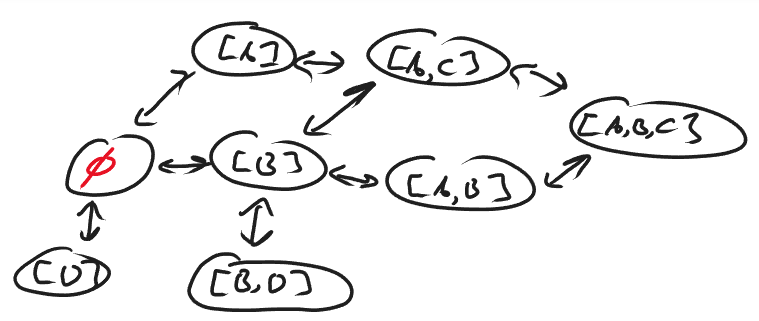
\includegraphics[width=0.5\linewidth]{resources/graph1.png}
    \caption{Example FSM Graph Of Archetypes During Runtime}
    \label{fig:graph1}
\end{figure}
                                                         
\begin{figure}[htbp]
    \centering
    \begin{verbatim}                                                                      
                     +---------+       +---------+                                  
                +--->|   [A]   |<----->|  [A,C]  |<---------+                        
          +-----+    +---------+       +---------+          |                        
          v                                    ^            v                        
     +---------+        +---------+            |         +---------+                   
     |   [0]   |<------>|   [B]   | <----------+         | [A,B,C] |                   
     +---------+        +---------+                      +---------+                   
         ^                  ^  ^                             ^                        
         |               +--+  |          +---------+        |                        
         v               v      +-------->|  [A,B]  +--------+                        
     +---------+     +---------+          +---------+                                 
     |   [D]   |     |  [B,D]  |                                                       
     +---------+     +---------+                                                              
    \end{verbatim}
    \caption{Dense ECS Architecture Table Example}
\end{figure}
                                                         
                                                         


As shown in Figure \ref{fig:graph1}, all graphs contain the empty set $\emptyset$ as a vertex. This is because all entities when initiated contain the the archetype with no components. As components get added to entities over their runtime, entities perform state transitions to their designated archetype.

It's important to note that this paper defines the serialization point to be the end of a tick and therefore entity transitions that occur during system runtime are invalid until the serialization point is reached. As such, an entities transition occurs once per tick to its final valid state. This means an entity could perform the transition, say $\{B,D\} \rightarrow \{A,B,C\}$ in one step, even though it passes through archetypes $[\{B\}, \{A,B\}]$ on the FSM. In the next tick, the edge $\{B,D\} \rightarrow \{A,B,C\}$ will be present. 

Archetype graphs display the following properties:

\begin{enumerate}
    \item All existing archetypes must have a path to vertex $\emptyset$.
    \item Components can appear multiple times.
    \item Archetypes can only appear once.
\end{enumerate}

There are a couple interesting things to notice in Figure \ref{fig:graph1}. Notice how there is no transition between state $[B,D]$ and $[D]$. This is because this graph represents a runtime of an ECS and while it is possible to transition between $[B,D] \leftrightarrow [D]$, it has yet to happen in this runtime context, and is therefore not required to exist. 

The component $C$ in Figure \ref{fig:graph1} is special in the regard that it is not adjacent to the $\emptyset$ vertex like the others. This does not mean that it is impossible to create an entity with only component $C$ but that the runtime has yet to have that situation occur.

To loop back to the proximity example in the introduction in section \ref{sec:fsm_arc}, by representing additions and deletions as runtime state transitions it should now be clear that large performance gains are achieved via these edges. Initially, the first entity that transitions between two states in the simulation will be slow because the edge between those two vertices must be made. Once that edge is made, it is cached and the deletion and transfer of an entity to another archetype drops from $O(N)$ to $O(1)$.

\subsubsection{Opertions On Entity FSM}
The following operations are all thread safe due to the scheduling algorithm explained in section \ref{sec:scheduling}. All implementation details are abstracted away except the operations directly done on the graph. 

\textbf{Entity Creation:} All entities when created start at the $\emptyset$ vertex. All entities that exist here are not queryable.

\textbf{Entity Component Addition: } Aside from the simple transition using an existing edge. When a component addition occurs, two operations are completed. Suppose the archetype we are currently in is at archetype $G$ and are attempting to add component $C$ to transition to $G \cup \{C\}$. The two operations presented are the lookup operation and the connection operation.

\begin{enumerate}
    \item If $G \cup \{C\} \not\in A$, then do step 2. Else do step 3.
    \item Create a new archetype $G \cup \{C\} \in A$. Apply component addition.
    \item Create the edge $G \leftrightarrow G \cup \{C\}$. Apply component addition.
\end{enumerate}

When considering concurrency, data invalidation can occur if the archetype transitions too early before the serialization point occurs. So these operations must be cached in some form. The simulation worlds handle this for us.

\textbf{Entity Component Deletion: } When an entity is marked to have a component deleted. The same algorithm is used in entity component addition. Both addition and deletion use the same transition function $\delta$ of the papers ECS definition.  

\textbf{Entity Deletion: }
When an entity is marked for deletion, the archetype has the choice to either delete it or wait to delete all entities together in a batch at some point in the future. Both of these strategies are thread safe. 

An important scenario to consider is what occurs when an archetype loses all its entities. While the archetype must be removed from the graph since no entities are there and to it'll keep it mathematically pretty, there is no need. In practice, theres a decently high probability that archetype will gain an entity again and deleting those edges will only slow down specific entity transition patterns. The memory usage of an empty archetype is inconsequential and therefore there is no real tradeoff of keeping it alive.

\subsection{Scheduling Systems}
\label{sec:scheduling}

Due to the nature that ECS follow principles in of data-oriented design, these architectures have an advantage in concurrency contexts. The following section is about an algorithm designed in this paper to schedule systems concurrently in such a way they produce one valid serialization point per tick. Therefore, this algorithm does not guarentee that all entities will enter a system all in any order or be processed in some order. Entities may be sent to the system in seemingly random orders.

\subsubsection{Scheduling Algorithm}
There are two classes of functions capable to be given to the scheduling algorithm from the user: functions that can be encapsulated by one archetype and functions that require multiple archetypes to process. In other words: systems where $\lambda_{\texttt{req}}$ is a subset of the archetype type set or where $\lambda_{\texttt{req}}$ is a superset of the archetype type set. Typically, superset type requests will be scheduled more serially since they "lock" more data within the real context. 

\begin{figure}[H]
    \begin{enumerate}
        \item For each $\lambda \in \Lambda$, do the following steps 2-3:
        \item Construct the set $x = \{\forall a \in A : \lambda_{req} \subseteq a \} \setminus \{\emptyset\}$.
        \item For each archetype in set $x$, mark that archetype to run $\lambda$.
        \item Schedule a unique thread for all archetypes.
        \item For each thread, run each system $\lambda$ that marked this archetype.
    \end{enumerate}
    \caption{Part 1 Scheduling}
\end{figure}

For the remaining systems unmarked, we sort them by the length of their archetype type set. This is done because the shortest ones have the best chance of running in parallel. The process from part 1 is reversed and archetypes are marked in a staging table. 

\begin{figure}[H]
    \begin{enumerate}
        \item For each leftover $\lambda \in \Lambda$, do the following steps 2-3:
        \item Use a set $a$, representing which archetypes have been marked this iteration.
        \item Loop through each archetype $g \in A$, do the following steps 4-5
        \item Skip $g$ if in $a$.
        \item If $g \subset \lambda\_{\texttt{req}}$ then add $g$ to $a$ and $g$ to $\lambda\_{\texttt{a}}$.
        \item After checking each archetype, reset $a$. Add 1 new row to the table.
        \item Go back to step 1 until the leftover $\lambda$ set is empty.
    \end{enumerate}
    \caption{Part 2 Scheduling}
\end{figure}

\textbf{Example:} The following is an example graph marked based on the algorithm above.

\begin{figure}[H]
    \centering
    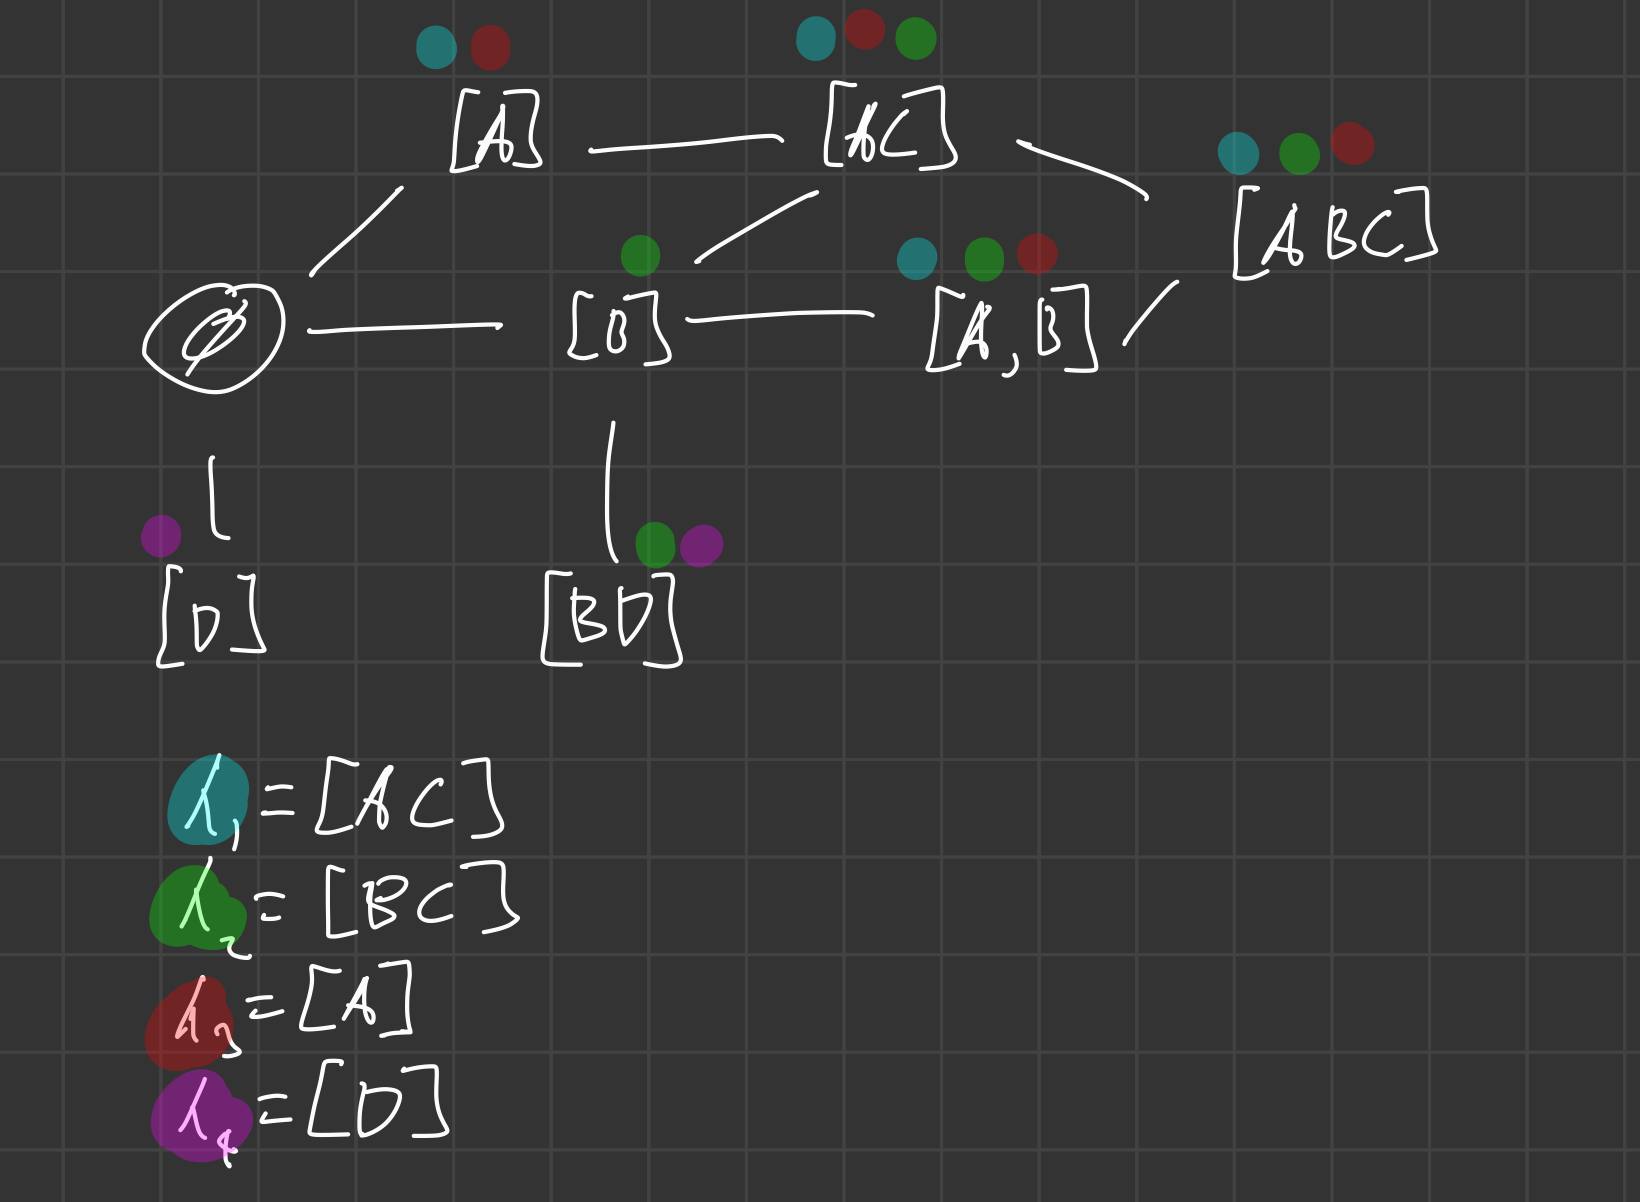
\includegraphics[width=0.5\linewidth]{resources/graph2.png}
    \caption{Example of a Scheduled Entity FSM Graph}
    \label{fig:graph2}
\end{figure}

The ECS in Figure \ref{fig:graph2} contains four systems: 

\begin{equation*}
    \Lambda = \begin{cases}
        \lambda_1 &= [A,C] \\
        \lambda_2 &= [B,C] \\ 
        \lambda_3 &= [A] \\ 
        \lambda_4 &= [D] \\ 
    \end{cases}
\end{equation*}

Notice how on any archetype vertex in this graph when there are multiple colors this signifies data contention. Depending on ECS access patterns, an ECS could possibly squeeze a bit more performance but for most cases it is unnecessary. Although, the GECS implemention does provide support for embarassingly parallel access patterns. So each $\lambda$ may also have some concurrency inside its own function.

\subsection{Entity Consolidation}
A key concept has been omitted thus far and that is entity consolidation. How, with these systems running concurrently, are entities transitioned between archetypes? It turns out, unlike entity modification which can be handled in parallel, component addition and deletion cannot be handled in any parallel contexts. The following sections contain a proof made for this paper and two workarounds are suggested.

\subsubsection{Entity Creation/Deletion Operations Leads To Tick Non-determinism}
\label{sec:proof1}
Suppose there exists two systems, systems A and B. The purpose of System A is to generate entities containing Component C and the purpose of System B is to consume entities that contain component C. In such an ECS runtime, that means entities are generated and transitioned to archetype $\{C\}$. Therefore the length of $\{C\}$ changes during the process of a tick. 

There are three cases in which System A and B interact:
\begin{enumerate}
    \item System A generates entities faster than B consumes
    \item System A generates entities at the same rate B consumes
    \item System A generates entities slower than B consumes
\end{enumerate}

Only in case 3 can the next tick occur. The nondeterminism introduced by allowing entity list mutations can cause program stalls such as in the manner proposed. And also in the context of a concurrent ECS, this can lead to deadlocks, livelocks, and data invalidation.

\subsubsection{Serializability And Ledger-Based Consolidation}
\label{sec:ledger}
In order to solve the problem of entity consolidation in any context the entity list must stay fixed. That means for each tick, no matter the deletion or additions performed, the entity set must stay the same until the tick is complete. As such, even if perfect concurrent entity consolidation is performed, the effort is still wasted. If the list of entities can only be mutated after the serialization point, then doing early consolidation is as if it was done now since only now can the affects of entity consolidation be seen. 

The GECS implementation proposes to use a ledger-based consolidation technique that caches mutation operations done on the entity list and applies these operations in order after the serialization point.

\subsubsection{Alternative To Ledger-Based Consolidation}
An alternative to the implementation GECS proposed is to add a constraint to $\lambda_{req}$ such that operations done where the queried archetype $a \not\subseteq \lambda_{req}$ makes them invalid. By doing so, it ensures that $\lambda$ will be scheduled by the scheduler to process $a$. 

This provides the unique opportunity that whenever working in the context of archetype $a$, all requests to create entities with archetype $a$ will be processed and all other requests ignored. In some ways, this alternative is more elegant than what GECS implemented. But this thought came too late in development and has some drawbacks. Mainly, having to know the set of components the system depends on before the system gets scheduled. I also theorize that this architecture will not be as performant as using a ledger because more archetypes will be contended and therefore some of the more concurrent work will be lost.

\subsubsection{$\delta$ Transition To $\emptyset$}
Going back to ledger-based consolidation. Since entity deletion causes an entity to transition to $\emptyset$, it is not parallelizable and the fact this entity is deleted must be stored in the ledger. After the serialization point occurs, the ECS will go and clean out all entities that are supposed to translate to the $\emptyset$ directly from the ledger. 

\subsubsection{$\delta$ Transition For Non-$\emptyset$ Operations}
Much like the transition to the $\emptyset$, since the entity is transitioning archetypes it is not parallelizable. The transition operation will be stored in the ledger. After the serialization point, then the ECS will perform the $\delta$ transitions. 
